\documentclass[liststotoc,bibtotoc,fontsize=14pt,]{scrreprt}
\usepackage[utf8]{inputenc} % Zeichenkodierung
\usepackage[ngerman]{babel} % neue deutsche Rechtschreibung
\usepackage{etoolbox}
\apptocmd{\thebibliography}{\raggedright}{}{}
\usepackage{graphicx}
\usepackage{url}
\usepackage[onehalfspacing]{setspace}
\usepackage{breakurl}
\usepackage{float}
\usepackage[table,xcdraw]{xcolor}
\usepackage{tabularx}
\usepackage[breaklinks]{hyperref}
\def\UrlBreaks{\do\/\do-}
\usepackage{tocloft}
\usepackage{chngcntr}
\usepackage{listings}
\usepackage{color}
\usepackage[parfill]{parskip}
\definecolor{lightgray}{rgb}{.9,.9,.9}
\definecolor{darkgray}{rgb}{.4,.4,.4}
\definecolor{purple}{rgb}{0.65, 0.12, 0.82}

\counterwithout{footnote}{chapter}

\deffootnote[2em]{2em}{2em}{%
	\makebox[2em][l]{\bfseries\thefootnotemark}}

\renewcommand{\cftchapdotsep}{\cftdotsep}
\renewcommand{\cftchapleader}{\cftdotfill{\cftchapdotsep}}
\usepackage{amsmath}
\usepackage[paper=a4paper,left=30mm,right=30mm,top=25mm,bottom=25mm]{geometry}
\usepackage[section]{placeins}
\usepackage[font=small,justification=justified]{caption}
\newcommand{\namesigdate}[3][Ort, Datum]{%
	\parbox{\textwidth}{
		\raggedleft #3 
		\vspace{2cm}
		
		\parbox{5cm}{
			\raggedright
			\rule{6cm}{1pt}\\
			#1 
		}
		\hfill
		\parbox{5cm}{
			\raggedright
			\rule{6cm}{1pt}\\
			#2
		}
	}
}


\newcommand*{\tabularwidth}{}
\newdimen\tabularwidth
\usepackage{minitoc}
\hypersetup{
	colorlinks,
	citecolor=black,
	filecolor=black,
	linkcolor=black,
	urlcolor=black
}


\title{Dokumentation Panoramafotografie}
\author{Sebastian Degner}

\begin{document}
	%\maketitle
	
	\begin{titlepage}
		\begin{center}
			\vspace{2cm}
			Dokumentation\\ \textbf{ Multishot-Technik in der digitalen Fotografie}\\ 
			\vspace{2,5cm}
			
\includegraphics[width=5cm]{HTWK_Logo_RGB-transparent_250.png}\\
			
			\vspace{2,5cm}
			\huge \textbf{\textsf{Dokumentation Panoramafotografie}} \\
			\vspace{3cm}
			\fontsize{15}{18} \textbf{Hochschule für Technik, Wirtschaft und Kultur
				Leipzig\\ Fakultät Informatik, Mathematik und Naturwissenschaften\\   Masterstudiengang Medieninformatik}\\
			\vspace{3cm}
		\end{center}
		\normalsize{
			\begin{tabular}{ll}
				Eingereicht von: & {Sebastian Degner} \\
				 & {Sebastian Knabe} \\
				Studiengang: & 15 MIM\\
				Eingereicht am: & 09. Dezember 2016 \\
			\end{tabular}\\
		}
		
	\end{titlepage}
	
	
	
	
	
	\tableofcontents
	\clearpage
	\listoffigures
	\addcontentsline{toc}{chapter}{Abbildungsverzeichnis}

	\chapter{Einleitung}
	\label{ch:einleitung}
		
	\chapter{Vorbereitung}
	\label{ch:vorbereitung}
	
	\section{Verwendete Kameratechnik}
	\label{sec:technik}
	
	\section{Justage des NPP}
	\label{sec:npp}
	
	\chapter{Aufnahmen}
	\label{ch:aufnahmen}
	
	\section{180$^\circ$ Panorama -- Speck\grq s Hof}
	\label{sec:specks}

	\subsubsection{Aufnahmeort und -idee}
	Charakteristisch für die Leipziger Innenstadt, ist die Vielzahl an Passagen und Durchgangshöfen, welche das Stadtild prägen. Die älteste, erhaltene Ladenpassage ist Speck\grq s Hof, welche zwischen 1908 und 1929, durch den Bau des Messehauses entstand. Den Namen erhielt die Passage aufgrund des Kaufhofes des Freiherrn von Speck, welches zuvor an dieser Stelle stand. Sie befindet sich an der Kreuzung Reichstraße / Grimmaische Straße, in direkter Nähe zur Nikolaikirche und ist mit dem Hansa Haus verbunden. In den Jahren 1993 bis 1995 wurde die Passage aufwendig restauriert. Heute bietet Speck\grq s Hof eine architektonische und gestalterische Mischung aus Vergangenheit und Gegenwart und ist beispielsweise durch Malereien und Plastiken der Künstler Bruno Griesel, Johannes Grützke und Moritz Götze verziert.
	
	\bigskip
	
	
	\subsubsection{Kameraeinstellungen}
	
	
	\section{180$^\circ$ Panorama -- Auerbachskeller}
	\label{sec:auer}

	\section{180$^\circ$ Nachtpanorama -- Richard Wagner Platz}
	\label{sec:wagner}
	
	\section{360$^\circ$ Panorama -- Augustusplatz}
	\label{sec:augustus}
	
	\section{360$^\circ$ Nachtpanorama -- Marktplatz}
	\label{sec:markt}
	
	\section{Kugelpanorama --  Mädler-Passage}
	\label{sec:kugel}
	
	\chapter{Stitching}
	\label{ch:stitiching}
	Für ein Panorama aufgenommene Einzelbilder werden in der digitalen Fotografie mittels des sogenannten Stitchings zu einem Gesamtbild zusammengesetzt. Um diesen Vorgang weitestgehend zu automatisieren, gibt es verschiedene kostenlose oder auch kostenpflichtige Programme. In dieser Arbeit wird dabei näher auf Photoshop (\ref{sec:photoshop}) und PTGui Pro (\ref{sec:ptgui}) eingegangen, da diese für die Erstellung und Bearbeitung im Vordergrund stehen. Eine freie Softwarealternative für das Stitchen ist Hugin, welches in dieser Arbeit allerdings keine Verwendung findet, da die eben genannten Alternativen bereits alle benötigten Funktionen beherrschen.
	
	\section{PTGUI Pro}
	\label{sec:ptgui}
	
	Beim Start der Anwendung öffnet sich ein simpel gestaltetes Fenster, welches in Abb. \ref{img:ptgui_step_1} zu sehen ist. Die Software ist übersichtlich in Tabs aufgebaut, welche nach dem Laden der Fotos verschiedene Optionen bereitstellen. Mit einem Klick auf \grqq{}Advanced\grqq{} lassen sich diese noch erweitern.
	\begin{figure}[H]
		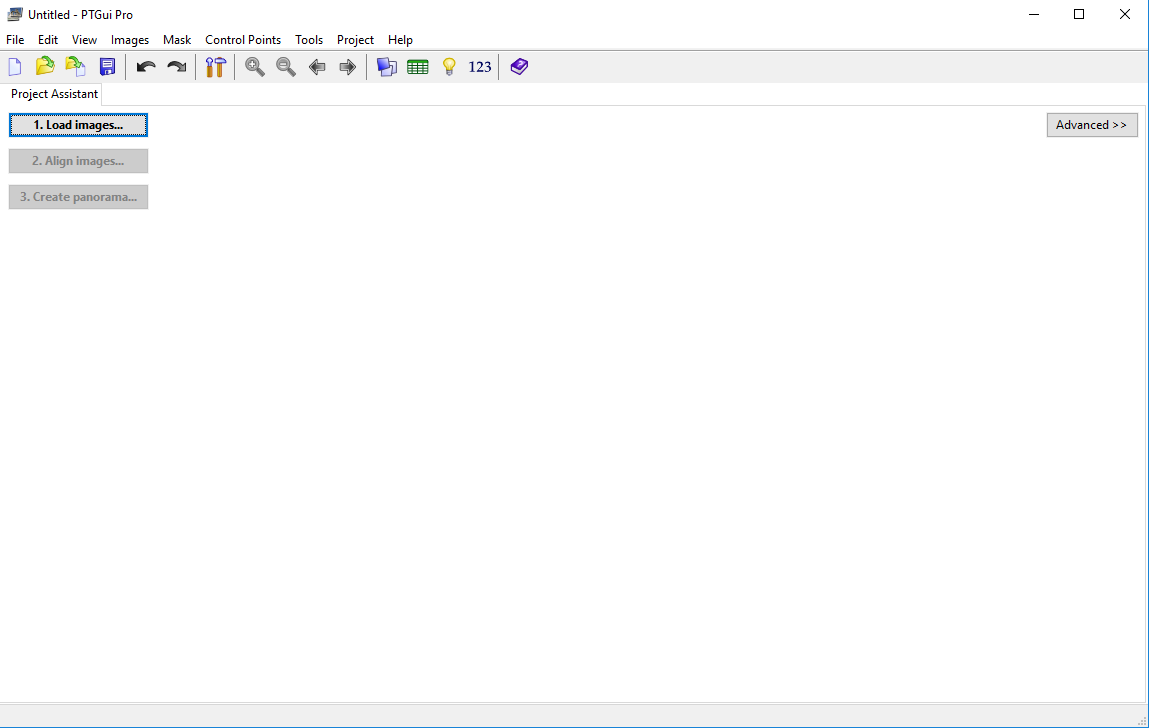
\includegraphics[width=\linewidth]{img/steps/PTGui_Step_1.PNG}
		\caption{PTGui Pro: Startfenster}
		\label{img:ptgui_step_1}
	\end{figure}
	\bigskip
	Über den \grqq{}Load images... -- Button\grqq{} lassen sich die Quellbilder zu einem neuen Projekt hinzufügen. Auch können an dieser Stelle Belichtungsreihen für die HDR--Entwicklung importiert werden. Anschließend werden die geladenen Bilder in dem bereits beschriebenen Startfenster angezeigt und die Einstellungsoptionen werden in Form von Tabs oberhalb angeordnet. 
	\begin{figure}[H]
		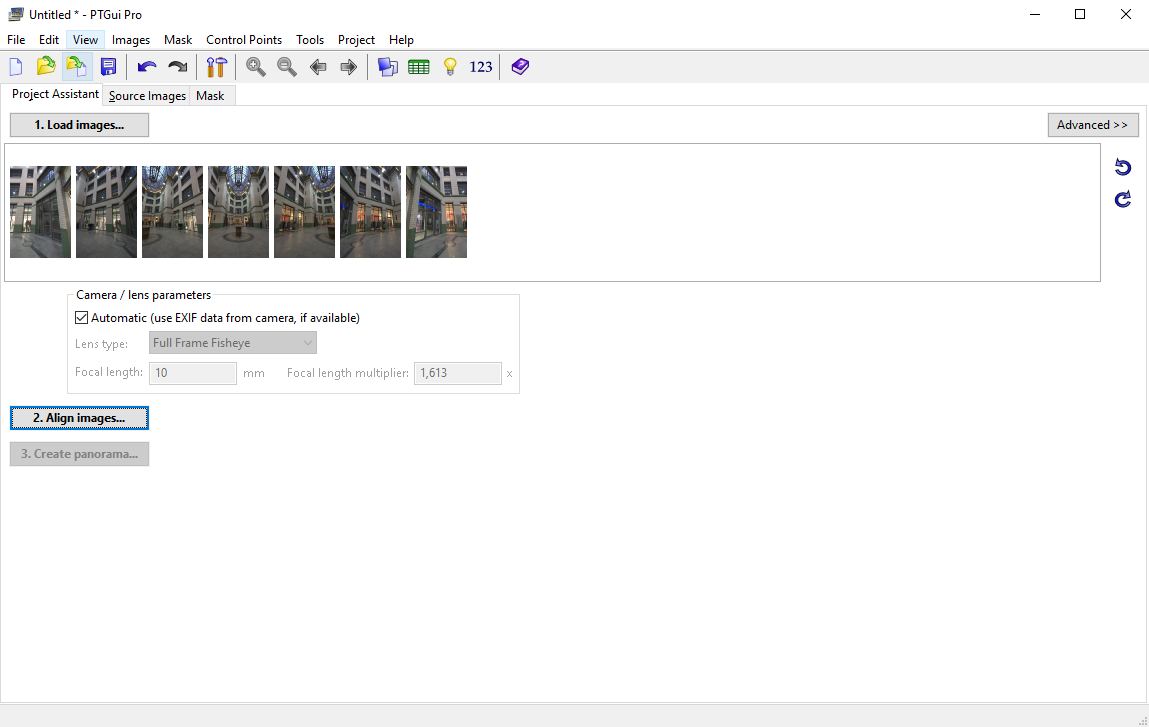
\includegraphics[width=\linewidth]{img/steps/PTGui_Step_2.PNG}
		\caption{PTGui Pro: Laden der Fotos}
		\label{img:ptgui_step_2}
	\end{figure}
	\begin{figure}[H]
		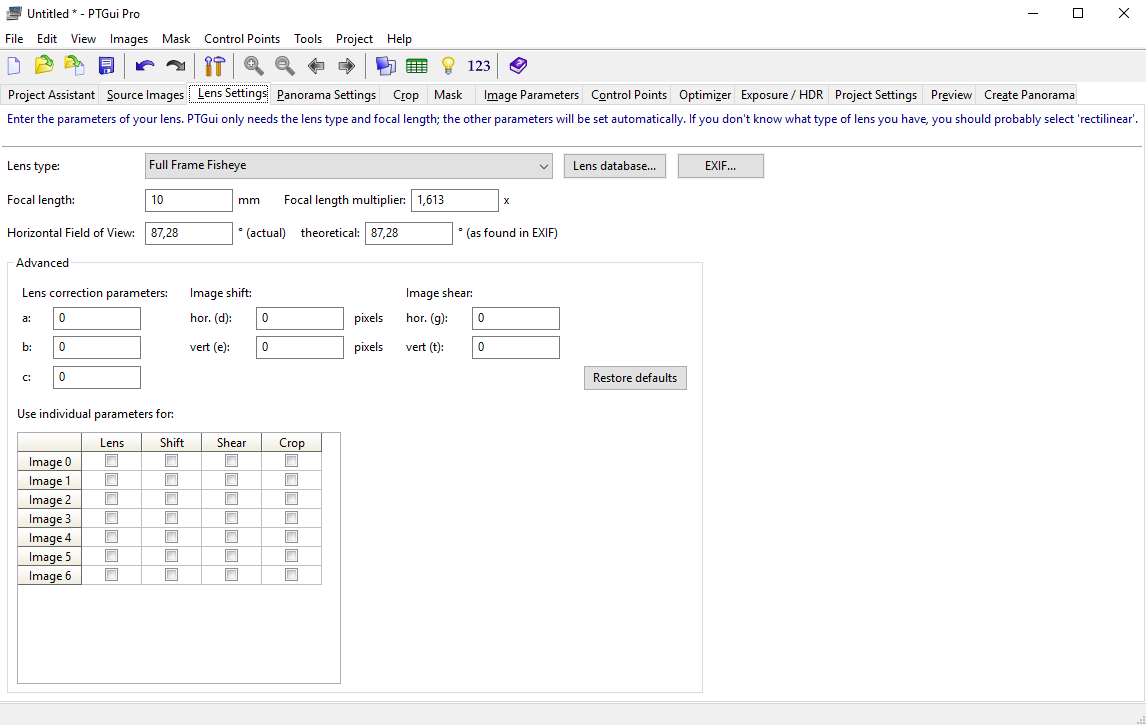
\includegraphics[width=\linewidth]{img/steps/PTGui_Step_3.PNG}
		\caption{PTGui Pro: Objektiveinstellungen}
		\label{img:ptgui_step_3}
	\end{figure}
	\begin{figure}[H]
		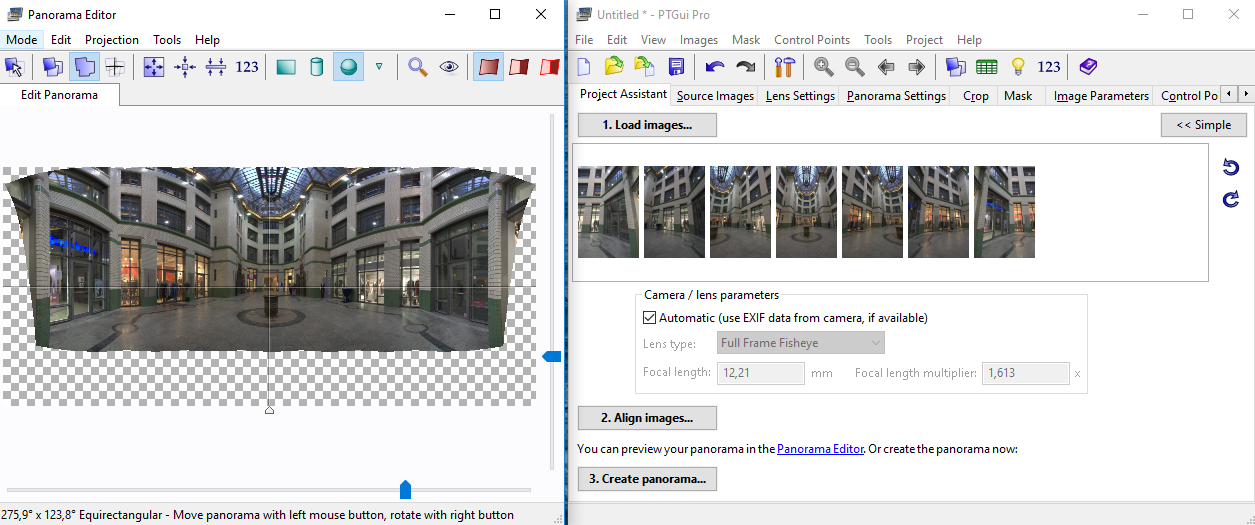
\includegraphics[width=\linewidth]{img/steps/PTGui_Step_4.PNG}
		\caption{PTGui Pro: Maskierung}
		\label{img:ptgui_step_4}
	\end{figure}
	\begin{figure}[H]
		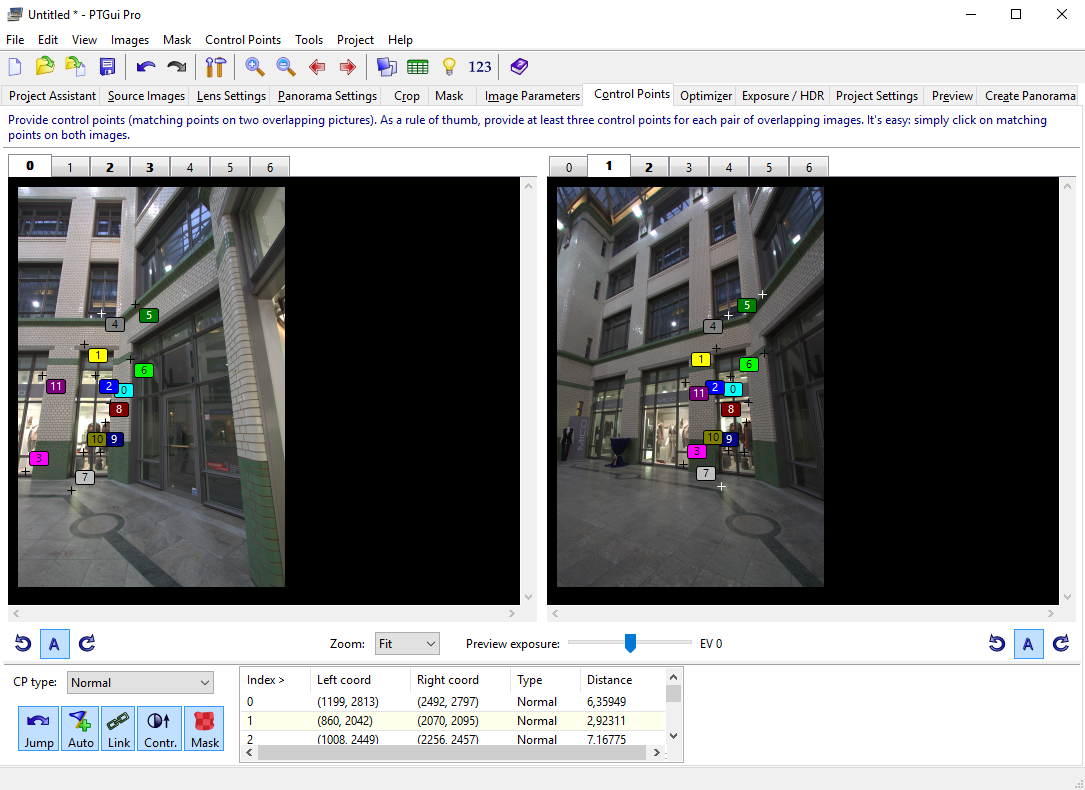
\includegraphics[width=\linewidth]{img/steps/PTGui_Step_5.PNG}
		\caption{PTGui Pro: Kontrollpunkte}
		\label{img:ptgui_step_5}
	\end{figure}
	\begin{figure}[H]
		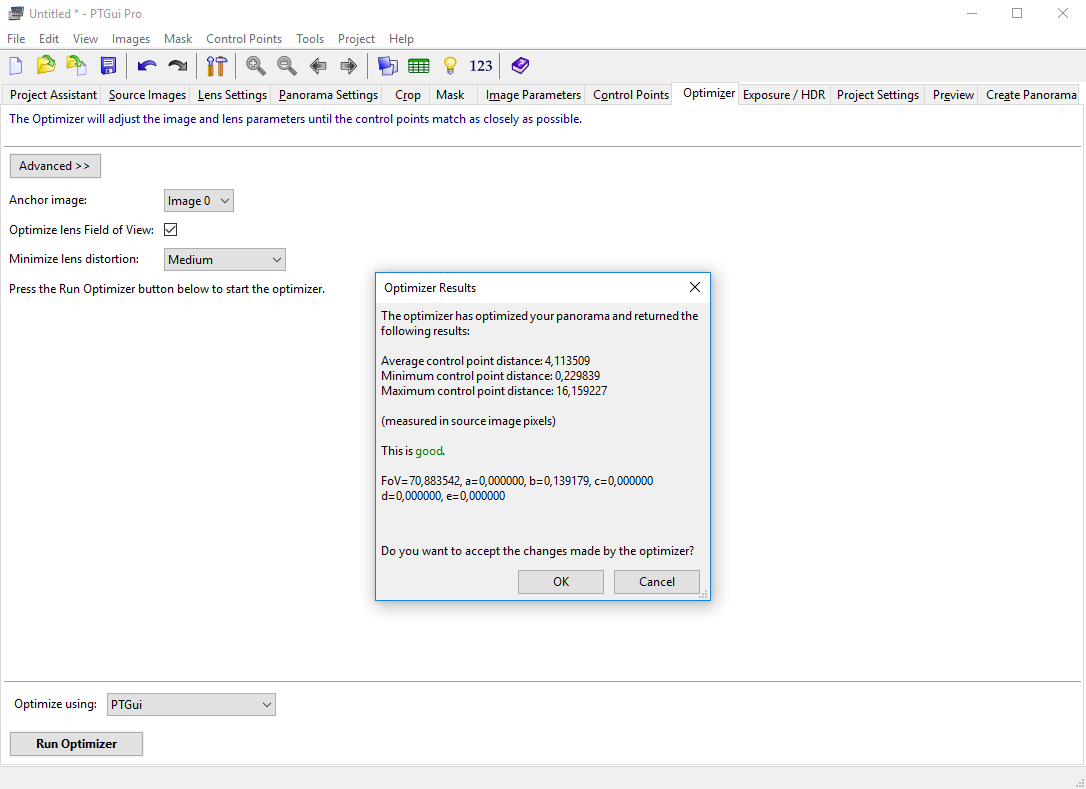
\includegraphics[width=\linewidth]{img/steps/PTGui_Step_6.PNG}
		\caption{PTGui Pro: Optimierung}
		\label{img:ptgui_step_6}
	\end{figure}
	\begin{figure}[H]
		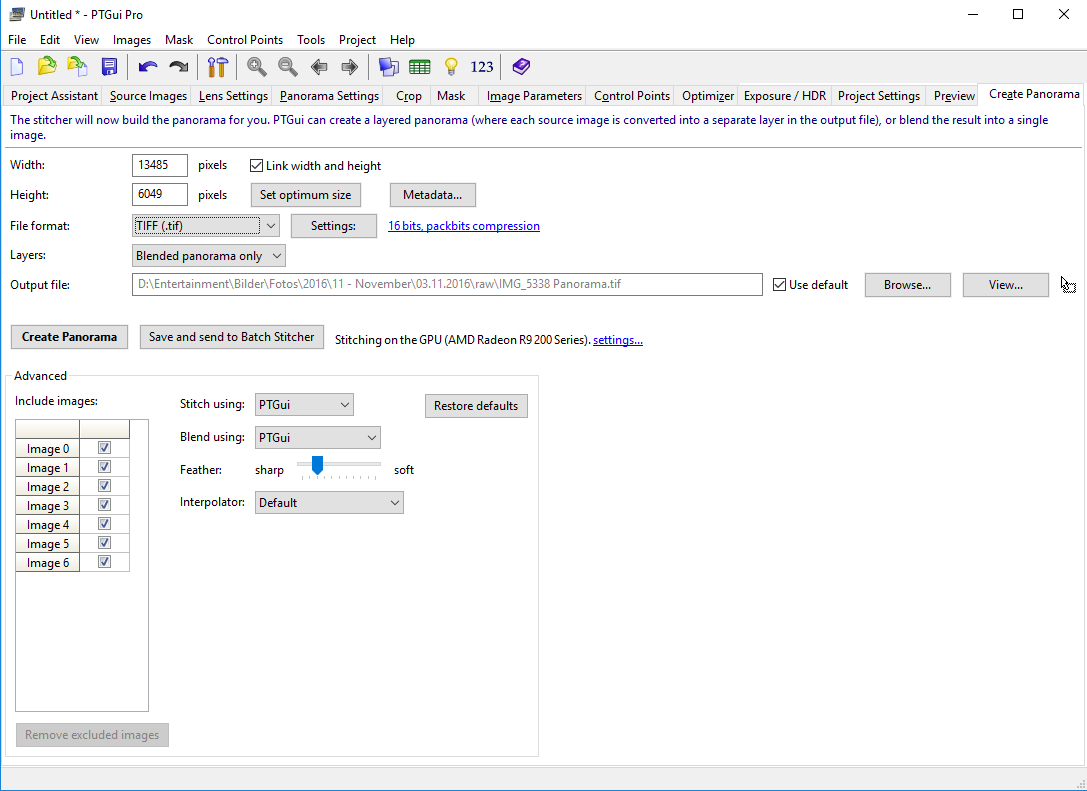
\includegraphics[width=\linewidth]{img/steps/PTGui_Step_7.PNG}
		\caption{PTGui Pro: Export}
		\label{img:ptgui_step_7}
	\end{figure}
	
	\section{Photoshop}
	\label{sec:photoshop}
	Stapelverarbeitung > Automatisch > fertig
	%TODO Bild
	
	\chapter{Nachbearbeitung}
	\label{ch:nach}
	
	\section{Lightroom}
	\label{sec:lightroom}
	
	\section{Photoshop}
	\label{sec:photo}
	

	
	\begin{thebibliography}{999}
	
		
	\end{thebibliography}
	
\end{document}